% "{'classe':('PSI'),'chapitre':'chs_leq','type':('td'),'titre':'Conception de la commande d’un robot chirurgical', 'source':'CCS PSI - 2015','comp':('C1-02','C2-04'),'corrige':False}"
%\setchapterimage{bandeau}
\chapter*{TD \arabic{cptTD} \\ 
Conception de la commande d’un robot chirurgical -- 
\ifprof Corrigé \else Sujet \fi}
\addcontentsline{toc}{section}{TD \arabic{cptTD} :
Conception de la commande d’un robot chirurgical -- 
\ifprof Corrigé \else Sujet \fi}

\iflivret \stepcounter{cptTD} \else
\ifprof  \stepcounter{cptTD} \else \fi
\fi

\setcounter{question}{0}
\marginnote{CCS PSI -- 2015.}
\marginnote[1cm]{
\UPSTIcompetence[2]{C1-02}
\UPSTIcompetence[2]{C2-04}}

\begin{marginfigure}[4cm]
\centering
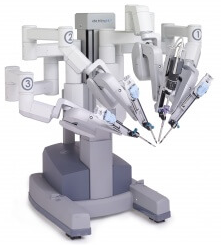
\includegraphics[width=\linewidth]{fig_00}
\end{marginfigure}





On s'intéresse au bras esclave d'un robot chirurgical. 
\begin{obj}
Justifier la structure du bras esclave par rapport au cahier des charges.
\end{obj}
\ifprof
\else
\begin{center}
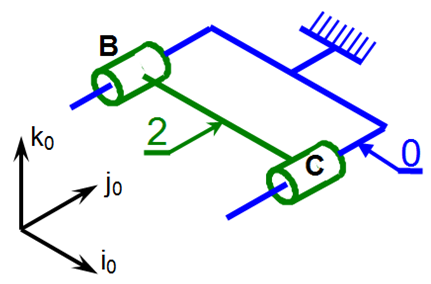
\includegraphics[width=\linewidth]{fig_02.png}
\end{center}

On donne le schéma cinématique partiel du bras esclave.

\begin{center}
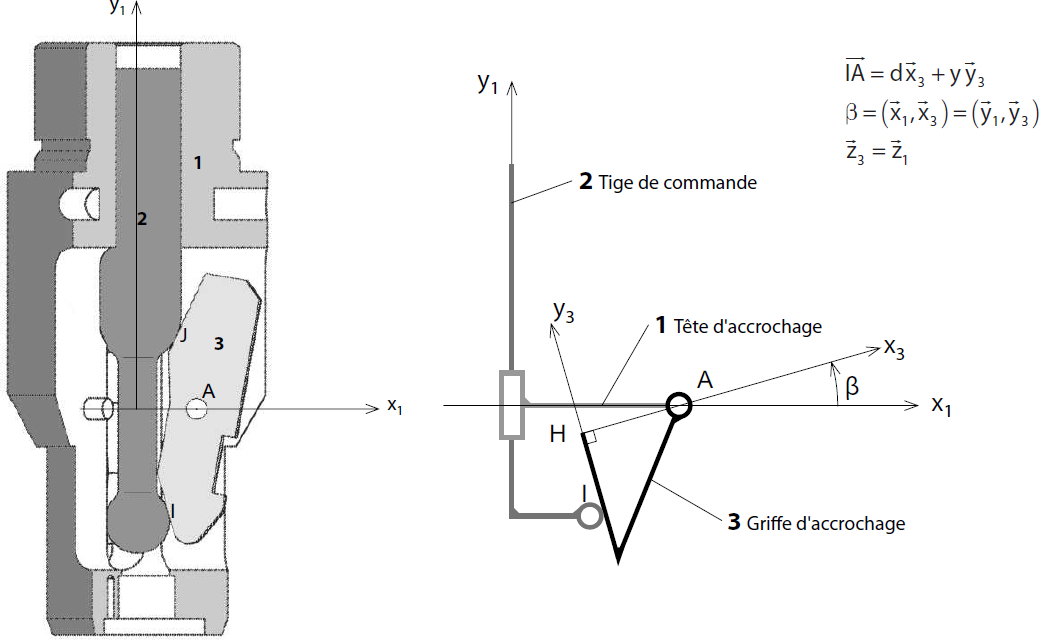
\includegraphics[width=\linewidth]{fig_01.png}
\end{center}


\begin{center}
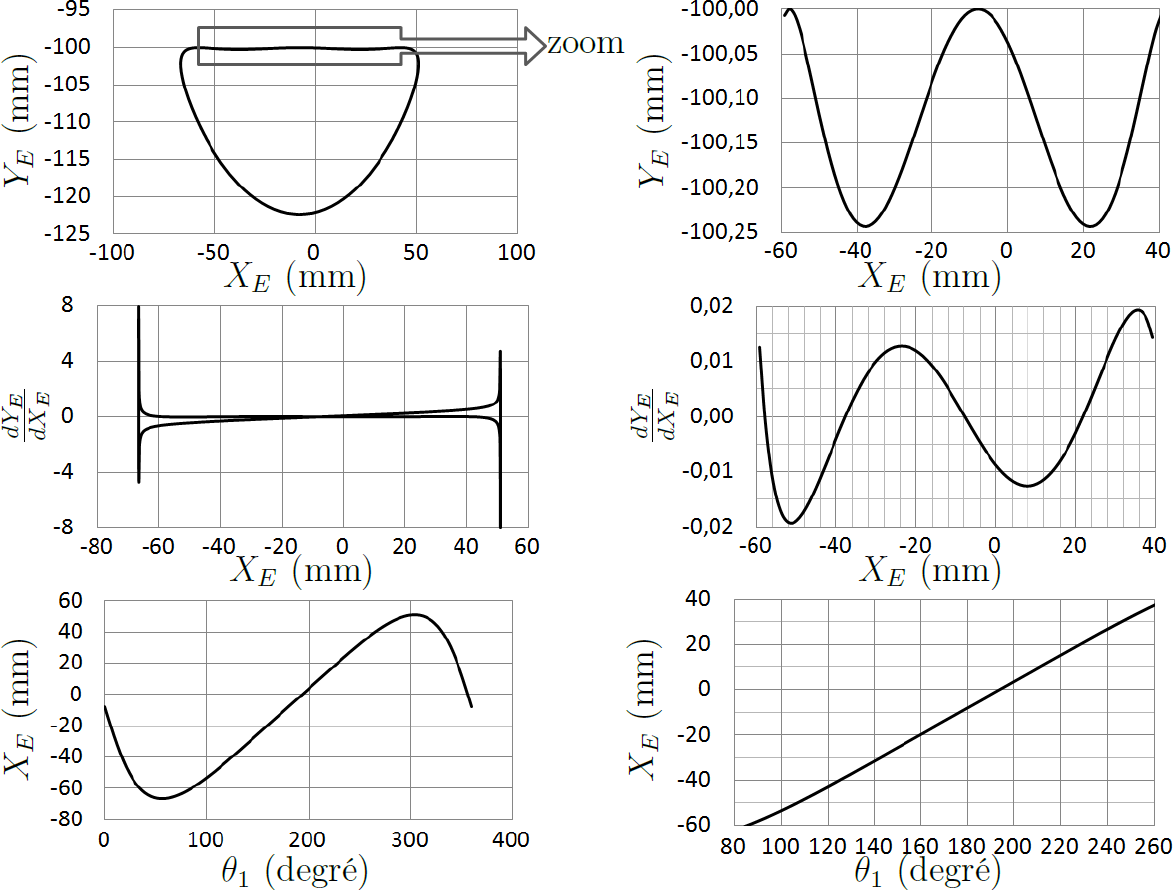
\includegraphics[width=\linewidth]{fig_03.png}
\end{center}


\begin{center}
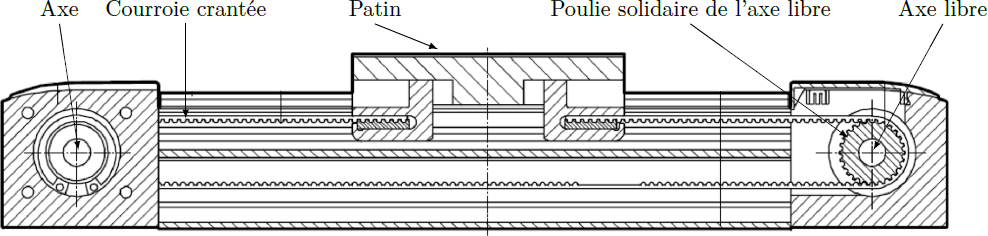
\includegraphics[width=\linewidth]{fig_04.png}
\end{center}

Le point $T$ est situé à l’intersection des axes $\axe{A'}{{x_0}}$ et  $\axe{P'}{{y_2}'}$. 
Le vecteur vitesse du point $T$ de 7’ par rapport à 0, noté $\vectv{T}{7'}{0}$, doit être colinéaire à 
$\vect{y_2}'$.
\fi

\question{En s’appuyant sur la figure précédente, calculer $\vectv{P'}{7'}{0}$ par dérivation du vecteur position.}
\ifprof
\begin{corrige}
\begin{center}
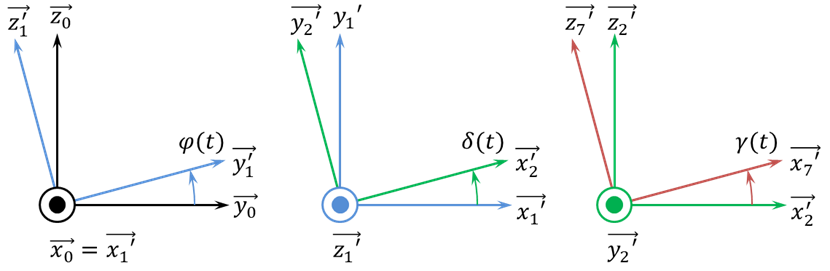
\includegraphics[width=\linewidth]{cor_01.png}
\end{center}
On a $\vectv{P'}{7'}{0} = \deriv{\vect{A'P'}}{\rep{0}}$
$ = \deriv{\vect{A'B'}+\vect{B'D'}+\vect{D'G'}+\vect{G'P'}}{\rep{0}}$
$ = \deriv{-h_1\vect{x_0}+h_2\vect{y_2'}-h_4\vect{x_0}-\lambda(t)\vect{y_2'}}{\rep{0}}$
$ = h_2\deriv{\vect{y_2'}}{\rep{0}}   -\lambda(t)\deriv{\vect{y_2'}}{\rep{0}}-\lambdap(t)\vect{y_2'}$

\end{corrige}
\else
\fi

\question{Exprimer $\vectv{T}{7'}{0}$ dans la base $\base{x_2'}{y_2'}{z_2'}$ en fonction des données de l’énoncé. Il est conseillé d’utiliser la relation de Varignon en passant par le point $P'$.}
\ifprof
\begin{corrige}
$\deriv{\vect{y_2'}}{\rep{0}} = \left( \dot{\delta}(t) \vect{z_1'}+\dot{\varphi}(t) \vect{x_1'}  \right)\wedge \vect{y_2'}$.

Au final, 
$\vectv{P'}{7'}{0}
=\left(h_2-\lambda (t)\right)
\left(-\dot{\delta}(t) \vect{x_2'}
+\varphip(t) \cos\delta(t)
\vect{z_1'}\right)
-\lambdap (t) \vect{y_2}'$.

De plus 
$\vectv{T'}{7'}{0} =\vectv{P'}{7'}{0} + \vect{TP'} \wedge \vecto{7'}{0}$
$=(h_2-\lambda(t))(
-\deltap(t) \vect{x_2}'
+\varphip(t)\cos\delta(t))
-\lambdap(t)\vect{y_2}'
+(h_2-\lambda(t))\vect{y_2}'\wedge (\deltap(t) \vect{z_1}'+\varphip(t) \vect{x_1}'+\gammap(t) \vect{y_2}')$
$=(h_2-\lambda(t))(-\deltap(t)\vect{x_2}'
+\varphi(t) \cos\delta(t) \vect{z_1}' )
-\lambdap(t) \vect{y_2}'+(h_2-\lambda(t)) \vect{y_2}'
\wedge\left(\deltap(t) \vect{z_1}'
+\varphip(t) \vect{x_1}'+\gammap(t)\vect{y_2}'\right)$
$=(h_2-\lambda(t))(-\deltap(t) \vect{x_2}'+\varphip(t)\cos\delta(t) \vect{z_1}' )-\lambdap(t) \vect{y_2}'+(h_2-\lambda(t))(\deltap(t) \vect{y_2}'\wedge\vect{z_1}'+\varphip(t) \vect{y_2}'\wedge\vect{x_1}' )$
$=(h_2-\lambda(t))(-\deltap(t) \vect{x_2}'+\varphip(t)  \cos\delta(t) \vect{z_1}' )-\lambdap(t) \vect{y_2}'+(h_2-\lambda(t))(\deltap(t) \vect{x_2}'
- \cos\delta(t)\varphip(t) \vect{z_1}' )$
$=-\lambdap(t) \vect{y_2}'$

\end{corrige}
\else
\fi


\question{Exprimer le torseur cinématique de $7’/0$ réduit en $T$, par ses composantes dans la base $\base{x_2'}{y_2'}{z_2'}$ et donner la liaison équivalente entre 7’ et 0 au point $T$.}
\ifprof
\begin{corrige}
$\vecto{7'}{0}=\left( \deltap\vect{z_1}'+\varphip \vect{x_1}'+\gammap\vect{y_2}' \right)$
$=(\deltap\vect{z_2}'+\varphip(\cos(\delta) \vect{x_2}'-\sin(\delta) \vect{y_2}' )+\gammap \vect{y_2}')$

La liaison équivalente 7’/0 est une liaison sphère -- cylindre de centre $T$ et de direction $\vect{y_2}'$.

\end{corrige}
\else
\fi

\question{Quelle exigence du cahier des charges (document réponse) justifie cette structure ? Expliquer sans calcul.}
\ifprof
\begin{corrige}
Exigence 1.5.
\end{corrige}
\else
\fi


\ifprof
\else
\begin{marginfigure}
\centering

\includegraphics[width=3cm]{Cy_06_01_TD_01_RobotChirurgical_qr}
\end{marginfigure}
\fi

